\documentclass[11pt]{article}
\usepackage[margin=1in]{geometry}
\usepackage{amsmath, amssymb, amsthm, enumerate}
\usepackage{graphicx,url, hyperref,framed, esint, color, tikz}

\setcounter{secnumdepth}{-2}

\begin{document}
\begin{flushright}
Alex Rich and Aaron Rosen\\
Engineering 155 \\ 
Final Project Status Report\\
November 21, 2015
\end{flushright}
\section{Project Status Report: A Robot Controlled Over The Internet}

***\\
Report should include:\\
A 4-page report (plus appendices) documenting your design at the midpoint. The status should include 
%\\- schematics of anything on a breadboard, 
\\- block diagrams of the logic on your FPGA, 
%\\- and an outline of the routines used on the Pi. 
\\ You should include as an appendix either your Verilog code or software that is mostly complete (but do not have to have both ready). 
\\- You must be ready to demonstrate some working hardware in the lab.
\\***

The team has made progress on a robotic vehicle that receives user input from a website and executes the commands. The website is hosted by an E155 Raspberry Pi2 Apache2 server, and contains a visual grid interface.  The grid represents different locations on the ground with respect to the vehicle.  To send the vehicle to the desired location, the user clicks on the corresponding point on the grid, which inputs commands into a buffer to be sent to the vehicle.  The Pi will parse the commands and send them wirelessly using a Belkin FT8001 Bluetooth dongle to a BlueSMiRF located on the vehicle.  The vehicle's controller (the E155 $\mu$Mudd board) reads these commands and executes them. An overview of this system is shown in Figure \ref{fig:sys}. Below we discuss the current status for each part (website, Pi, FPGA, vehicle, new hardware) in detail.

\subsection{Website}
The website currently contains a visual user interface that contains instructions for use, a grid on which to input locations for the robot to maneuver to, a list of the locations currently buffered for sending, and an option to clear the buffer. The code for the website is shown in Appendix A. The website was built using HTML, Javascript, and Bootstrap CSS. 

\subsection{Raspberry Pi 2}
The Pi hosts the website. Upon clicking in a grid space, the page's javascript calculates the left and right tread speeds and duration of movement required to get the tank to move from its original position to the new position. Next, the javascript makes an HTTP GET request to the inputChars resource of the Pi. When the request is completed, the page updates, either submitting the next command in the buffer or waiting for another input from the user.

After receiving a GET request, the common gateway interface (CGI) reads the input parameters and calls a Python script. The Python script utilizes the \verb.bluetooth. module to allow sending data using the bluetooth dongle. Since the robot has a constant bluetooth device address, this address is hard coded into the Python script. When called, the python script sends the commands, one at a time, to the robot. Currently, the system sleeps for an amount of time to theoretically give the vehicle enough time to move. However, in the future, the Pi will wait for acknowledgement from the FPGA. The code on the Pi is shown in Appendix B. In summary, here is the order in which the Pi responds to user input.

\begin{figure}
\begin{center}
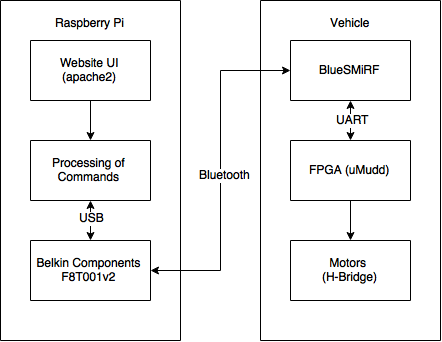
\includegraphics[width=0.7\textwidth]{E155System}
\end{center}
\caption{An overview of the system. The system is comprised of two major subsystems: the Raspberry Pi 2 controller and the vehicle, which is controlled by the $\mu$Mudd board.}
\label{fig:sys}
\end{figure}

\subsection{FPGA}
The FPGA reads data from a BlueSMiRF using UART hardware coded in SystemVerilog and then processes and executes the command.  It is constructed as a controller-datapath pair with three main submodules - receiveMSG, executeCommand, and sendAck.  The SystemVerilog code running on the FPGA is shown in Appendix C. The FPGA and BlueSMiRF are the only two electrical components on the breadboard. The schematic is shown in figure \ref{fig:breadboard}

The clock used to interface with the BlueSMiRF is implemented using a PLL that oversamples the 112.5 Kbaud frequency by a factor of 8.  This oversampler determines if there is an incoming message.  The actual sampling of the BlueSMiRF's TX line is accomplished using a frequency divider that allows for sampling at the correct rate.  The divider's phase can be controlled in order to ensure that the sampling of the line is as close to the center of the transmission's clock as possible.  As there are three characters in each command, the code holds the system in the receiveMSG state until all three characters have been loaded.

The FPGA executes the command received by controlling the two motors via the H-Bridges on the $\mu$Mudd board. Each command consists of a PWM setting for each motor and a duration for which the motors should be running.  A counter is used to create a reference clock for PWM; the power levels are referenced against this counter to determine the correct duty cycle.  To prevent the vehicle from running indefinitely, the timer stops incrementing when the requested duration is reached, and a signal is output that is used to cut power to the motors.  Each LSb of the duration char corresponds to roughly one-tenth of a second duration.

Once the requested duration has been reached and power to the motors cut, the FPGA transmits the character 'A' back to the BlueSMiRF as an ACK code.  After this ACK has been sent, the FPGA will cycle around to the receiveMSG state again.

At this time, the $\mu$Mudd board interfaces with the BlueSMiRF.  All parts of the code have been written; however there are still critical bugs in the code to be worked out.  The receiveMSG and controller modules have been independently verified in ModelSim.  The other two main submodules will be independently verified shortly, and then the whole system will be tested together.




\subsection{Vehicle}
All of the parts for the vehicle have been ordered and received. The vehicle has yet to be assembled, as there will be no machining or fabrication involved at this point.

\begin{figure}
\begin{center}
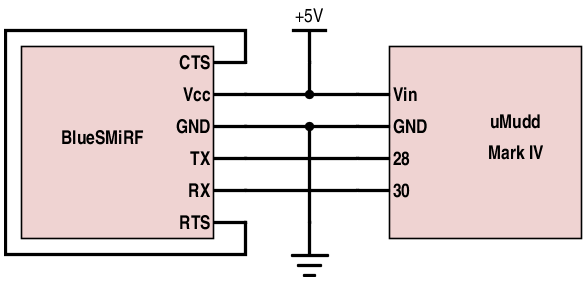
\includegraphics{breadboard}
\end{center}
\caption{The schematic of the circuit on the breadboard. In simple applications, the CTS and RTS pins of the BlueSMiRF are connected together, and the only pins that are connected to the FPGA are TX and RX.}
\label{fig:breadboard}
\end{figure}



\section{Appendix A: Website}
\subsection{Code}

\subsection{Result}

\section{Appendix B: Raspberry Pi2 Code}

\section{Appendix C: SystemVerilog Code on FPGA}
\small
\begin{verbatim}
module VehicleControl(input logic clk,
							 input logic RX,
							 output logic TX,
							 output logic[1:0] HL,HR);
		//top level module
		logic[7:0] lmotor,rmotor,dur;
		logic loadStart,loadComplete;
		logic executeStart,executeComplete; //executeStart should pulse when starting rather than staying high
		logic ackStart,ackSent;
		logic pllclk;
		logic reset,locked;
		
		PLLclk pll(reset,clk,pllclk,locked);
		
		controller control(clk,loadComplete,executeComplete,ackSent,loadStart,executeStart,ackStart); //datapath controller
		
		receiveMSG RXin(clk,pllclk,RX,loadStart,lmotor,rmotor,dur,loadComplete);
		executeCommand executor(clk,(loadComplete | executeStart),loadStart,lmotor,rmotor,dur,executeComplete,HL,HR);
		sendAck TXout(pllclk,ackStart,ackSent,TX);
		
endmodule

module controller(input logic clk,
						input logic loadComplete,
						input logic executeComplete,
						input logic ackSent,
						output logic loadStart,
						output logic executeStart,
						output logic ackStart);
	//datapath controller
	reg[2:0] state;
	logic execute,executeDelayed;
	always_ff @(posedge clk)
		begin
			case(state)
				3'b001:	begin
								if(loadComplete) 		state<=3'b010; //state becomes execute
								else						state<=3'b001; //state remains load
							end
				3'b010:	begin
								if(executeComplete) 	state<=3'b100; //state becomes ack
								else						state<=3'b010; //state remains execute
							end
				3'b100:	begin
								if(ackSent) 			state<=3'b001; //state becomes load
								else						state<=3'b100; //state remains ack
							end
				default: 								state<=3'b001; //default to load
			endcase
		end
	assign {ackStart,execute,loadStart}=state; //delegate signals accordingly
	flop executeDelay(clk,execute,executeDelayed);
	assign executeStart = execute & ~ executeDelayed;
endmodule

module receiveMSG(input logic clk,PLLclk,
				  input logic RX,loadStart,
				  output logic[7:0] lmotor,rmotor,dur,
				  output logic loadComplete);
	//top level for message recive subsystem
	logic[7:0] char;
	logic RXdone;
	logic resetTrigger;
	UARTRX receiveChar(clk,PLLclk,RX,loadStart,char,RXdone);
	shift3rst receiveCtr(loadStart,RXdone,resetTrigger,loadComplete);
	always_ff @(posedge RXdone)
		begin
			if(loadStart) {lmotor,rmotor,dur}={rmotor,dur,char};
		end
	flop #(1) loadCompleteDelay(clk,loadComplete,resetTrigger);
endmodule

module executeCommand(input logic clk,
							 input logic resetDur,presetDur,
							 input logic [7:0]lmotor,rmotor,dur,
							 output logic executeComplete,
							 output logic [1:0] HL,HR);
	//top level for message execute subsystem
	logic LPWM,RPWM;
	
	durcheck duration(dur,clk,resetDur,presetDur,executeComplete);
	pwm lmotorPWM(lmotor[6:0],clk,resetDur,LPWM);
	pwm rmotorPWM(rmotor[6:0],clk,resetDur,RPWM);
	hBridgeIn LHbridge(LPWM,executeComplete,lmotor[7],HL);
	hBridgeIn RHbridge(RPWM,executeComplete,rmotor[7],HR);
endmodule

module sendAck(input logic clk,
					input logic ackStart,
					output logic ackSent,
					output logic TX);
	//top level for ack send subsystem
	UARTTX sendChar(clk,ackStart,TX,ackSent);
	
endmodule

module UARTTX(input logic clk,
				  input logic ackStart,
				  output logic TX,
				  output logic msgSent);
	//UART TX Pin
	//ACK is "A" (0x41), msg is 11'b0_0100_0001_11 = 11'b001_0000_0111 = 11'h107
	logic resetTrigger;
	logic clk2;
	logic[10:0]msg;
	logic[3:0]count; //keeps track of the number of bits sent
	slowclk baudrate(clk,1'b1,clk2);
	always_ff @(posedge clk2)
		begin
			if(ackStart) {msg[9:0],msg[10]}={msg}; //this is an 11-bit shift register
			else {msg[9:0],msg[10]} = {10'h107,1'h0};	//reset message loop to default position
		end
	assign TX = msg[0];
	timer #(4) bitCount(clk2,resetTrigger,count);
	assign msgSent = (count == 11); //message send high after 11th bit sent
	flop #(1) msgSentDelay(clk,msgSent,resetTrigger);
	
endmodule

module UARTRX(input logic clk,PLLclk,
			  input logic RX,
			  input logic loadStart,
			  output logic[7:0] char,
			  output logic done);
	//UART RX Pin
	logic[3:0] validCheck;
	logic valid;
	logic UARTclk;
	logic[1:0] stopBits;
	logic resetTrigger;
	logic startBit;
	logic loadStartDelayed,doneDelayed;
	
	always_ff @(posedge clk,posedge done)
		begin
			if(done) valid <= 0;
			else valid <= valid | (~|(validCheck));
		end
	shift4 sampler(RX,PLLclk,validCheck);
	slowclk baudrate(PLLclk,valid,UARTclk);
	always_ff @(posedge UARTclk,posedge resetTrigger)
		begin
			if(resetTrigger) {done,startBit,char,stopBits} = 12'h001;
			else {done,startBit,char,stopBits}={startBit,char,stopBits,RX}; //this is an 12-bit shift register	
		end
	delay #(1) doneDelay(clk,done,doneDelayed);
	delay #(1) loadStartDelay(clk,loadStart,loadStartDelayed);
	assign resetTrigger = doneDelayed | (~loadStartDelayed & loadStart);
endmodule

module hBridgeIn(input logic pwr,done,direction,
				 output logic[1:0] out);
	//cuts power to H-Bridge when done is asserted
	logic[1:0]sig;
	assign sig[0]=0;
	assign sig[1] = pwr & ~done;
	assign out = direction?{sig[0],sig[1]}:sig; //direction is sign in sign/mag number
endmodule

module pwm(input logic [6:0] power,
		   input logic clk,reset,
		   output logic wave);
	//Takes in an input signal and outputs corresponding PWM signal
	logic [6:0] count;
	timer #(7) pwmTimer(clk,reset,count);
	assign wave = (power > count);
endmodule

module durcheck(input logic[7:0] dur,
				input logic clk,reset,preset,
				output logic done);
	//checks the duration and cuts power to the wheels when done
	logic[29:0] durTime;
	always_ff @(posedge clk,posedge reset,posedge preset)
		begin
			if(reset) durTime <=0;
			else if(preset) durTime <= {dur,22'b0};
			else if(done) durTime <= durTime;
			else durTime <= durTime + 1'b1;
		end
	assign done = &(dur & durTime[29:22]);
endmodule

module shift3rst(input logic in,clk,reset,
			  output logic out);
	//3-register shift register with reset
	logic d1,d2;
	always_ff @(posedge clk,posedge reset)
		if(reset)
			begin
				d1 <=0;
				d2 <=0;
				out <=0;
			end
		else
			begin
				d1<=in;
				d2<=d1;
				out<=d2;
			end
endmodule

module shift4(input logic in,clk,
			  output logic[3:0] out);
	//4-register shift register, outputs all shifted bits		  
	always_ff @(posedge clk)
		begin
			out[0]<=in;
			out[1]<=out[0];
			out[2]<=out[1];
			out[3]<=out[2];
		end
endmodule

module slowclk(input logic clk,valid,
			   output logic clk2);
	//creates a second slow timer that is reliant on valid for centering
	logic [2:0]count;
	always_ff  @(posedge clk)
		begin
			if(valid) count <= count + 3'h1; //if the signal is valid, increment the counter normally
			else
				begin  //if the signal is not valid, hold the slow clock right before the transition
					count[2] <= 0;
					count[1] <= 1;
					count[0] <= 1;
				end
		end
	assign clk2=count[2];
endmodule

	
module timer #(parameter WIDTH=8)
			  (input logic clk,reset,
			   output logic [WIDTH-1:0] timeout);
	//a WIDTH-bit timer
	always_ff @(posedge clk,posedge reset)
		begin
			if(reset) timeout <= 0;
			else timeout <= timeout + 1'b1;
		end
endmodule

module flop #(parameter WIDTH=1)
				 (input logic clk,
				  input logic [WIDTH-1:0] d,
				  output logic [WIDTH-1:0] q);
	always_ff @(posedge clk)
		begin
			q <= d;
		end
endmodule 

module delay #(parameter WIDTH=1)
				 (input logic clk,
				  input logic [WIDTH-1:0] d,
				  output logic [WIDTH-1:0] q);
				  
	logic[WIDTH-1:0] p;
	always_ff @(posedge clk)
		begin
			p <= d;
			q <= p;
		end
endmodule

\end{verbatim}


%
%\section{Bill of Materials}
%
%\centering
%\begin{tabular}{|l|l|l|l|}
%\hline
%\multicolumn{1}{|c|}{\textbf{Item}} & \multicolumn{1}{c|}{\textbf{Description}}               	& \multicolumn{1}{c|}{\textbf{Source}} & \multicolumn{1}{c|}{\textbf{Cost}} \\ \hline
%Tracked Vehicle 			&										&							&	\\
%			Chassis Kit	& Chassis for the tank, includes treads and frame.    	& Amazon 					& 15.39                          	\\ \hline
%Tamiya 70168				& Gives tank flexibility to turn by controlling each     	& 							& \\
%Double Gearbox			& tread independently.						& Amazon		               			& 11.99                             	\\ \hline
%$\mu$Mudd Board                	& Controls the vehicle                                                 & E155                                 		& 0.00                               	\\ \hline
%			                      	& Provides website interface and sends commands 	&							&\\
%Raspberry Pi 2			    	& to vehicle             							& E155                                 		& 0.00                               	\\ \hline
%                        				& Wirelessly communicate via Bluetooth between  	&							&\\
%2X BlueSMiRF				& Pi and $\mu$Mudd board. 					& E155                                		& 0.00                               	\\ \hline
%2X TrustFire 14500			& Li Ion battery, 3.7 V 						& Aaron Rosen					& 0.00				\\ \hline
%\end{tabular}

\end{document}


























